\chapter{Introduction}


***
plan

intro - general trend towards computer model so no animal/human cruelty or tests
comp power not yet there
tailored medicine
mc method powerful techniques

move onto mc methods
history
what are they
examples
applications

thesis outline
signpost chapters

***

\section{Thesis Outline and Objective}

This thesis concerns the development of advanced 3D light transport algorithm for various biophotonic and medical applications.
The technique that is adopted to calculate the light transport for the majority of the thesis is the \gls*{mcrt} method.
This method allows the tracking of photon packets through simulated 3D mediums, with the inclusion of multiple anisotropic scattering events along with the modelling of various other micro-physics that light may undergo in a medium.


This chapter details the background to the Monte Carlo method and its various application to a myriad of different fields.

\section{Monte Carlo Method}\label{sec:mcmethod}
The Monte Carlo method is a numerical analysis technique based upon random numbers, which are used to calculate unknown variables in problems~\cite{cashwell1959practical,rogers1990monte}. 

The earliest use of the method is in Buffon's needle experiment of the 18$^{th}$ century~\cite{badger1994lazzarini,beckmann2015history,buffon1785histoire}. Buffon asked the question;

\medskip

``Suppose we have a floor made of parallel strips of wood, each the same width, and we drop a needle onto the floor. What is the probability that the needle will lie across a line between two strips?''

\medskip

The solution to this question is:
for a needle length \textit{l}, strip separation \textit{s}, where \textit{x} is the distance from the needle to the closest line, and $\theta$ is the angle of the needle with respect to the wood strips. Then using a simple geometrical argument, a needle crosses a strip if $x \leq \tfrac{l}{2} sin \theta$.

$x$ is distributed uniformly in [0, $\tfrac{s}{2}$], and $\theta$ in [0, $\tfrac{\pi}{2}$]. Therefore the probability density function for $x$ is $p(x)=\tfrac{2}{s}$, and $\theta$ is $p(\theta) = \tfrac{2}{\pi}$. The \gls*{pdf}, is a function of a variable that gives probability for a variable to a take a given value. The \gls*{pdf} is normalised over the whole range of the variable, in this case $x$, and $\theta$.
Thus, as $x$ and $\theta$ are independent variables, giving a joint probability of $p(x,\theta) = \tfrac{4}{s \pi}$.
So the probability of a needle of length $l$ ($l<s$) is:

\begin{equation}
P=\int_0^{\frac{\pi}{2}}\int_0^{\frac{l}{2}sin\theta}\frac{4}{s\pi}\ dx\ d\theta = \frac{2 l}{s \pi}\label{eqn:buffon}
\end{equation}


\Cref{eqn:buffon} can be used to carry out a Monte Carlo estimation of $\pi$. A simple rearrangement yields: $\pi = \tfrac{2l}{sP}$ where P is the ratio of needles crossing the line to the total number dropped. Laplace was the first to suggest that Buffon's needle experiment could be used to estimate $\pi$~\cite{beckmann2015history}. 
\Cref{fig:buffon-needle} shows an example of a simulation of Buffon's needle experiment.

\begin{figure}[!htb]
\centering
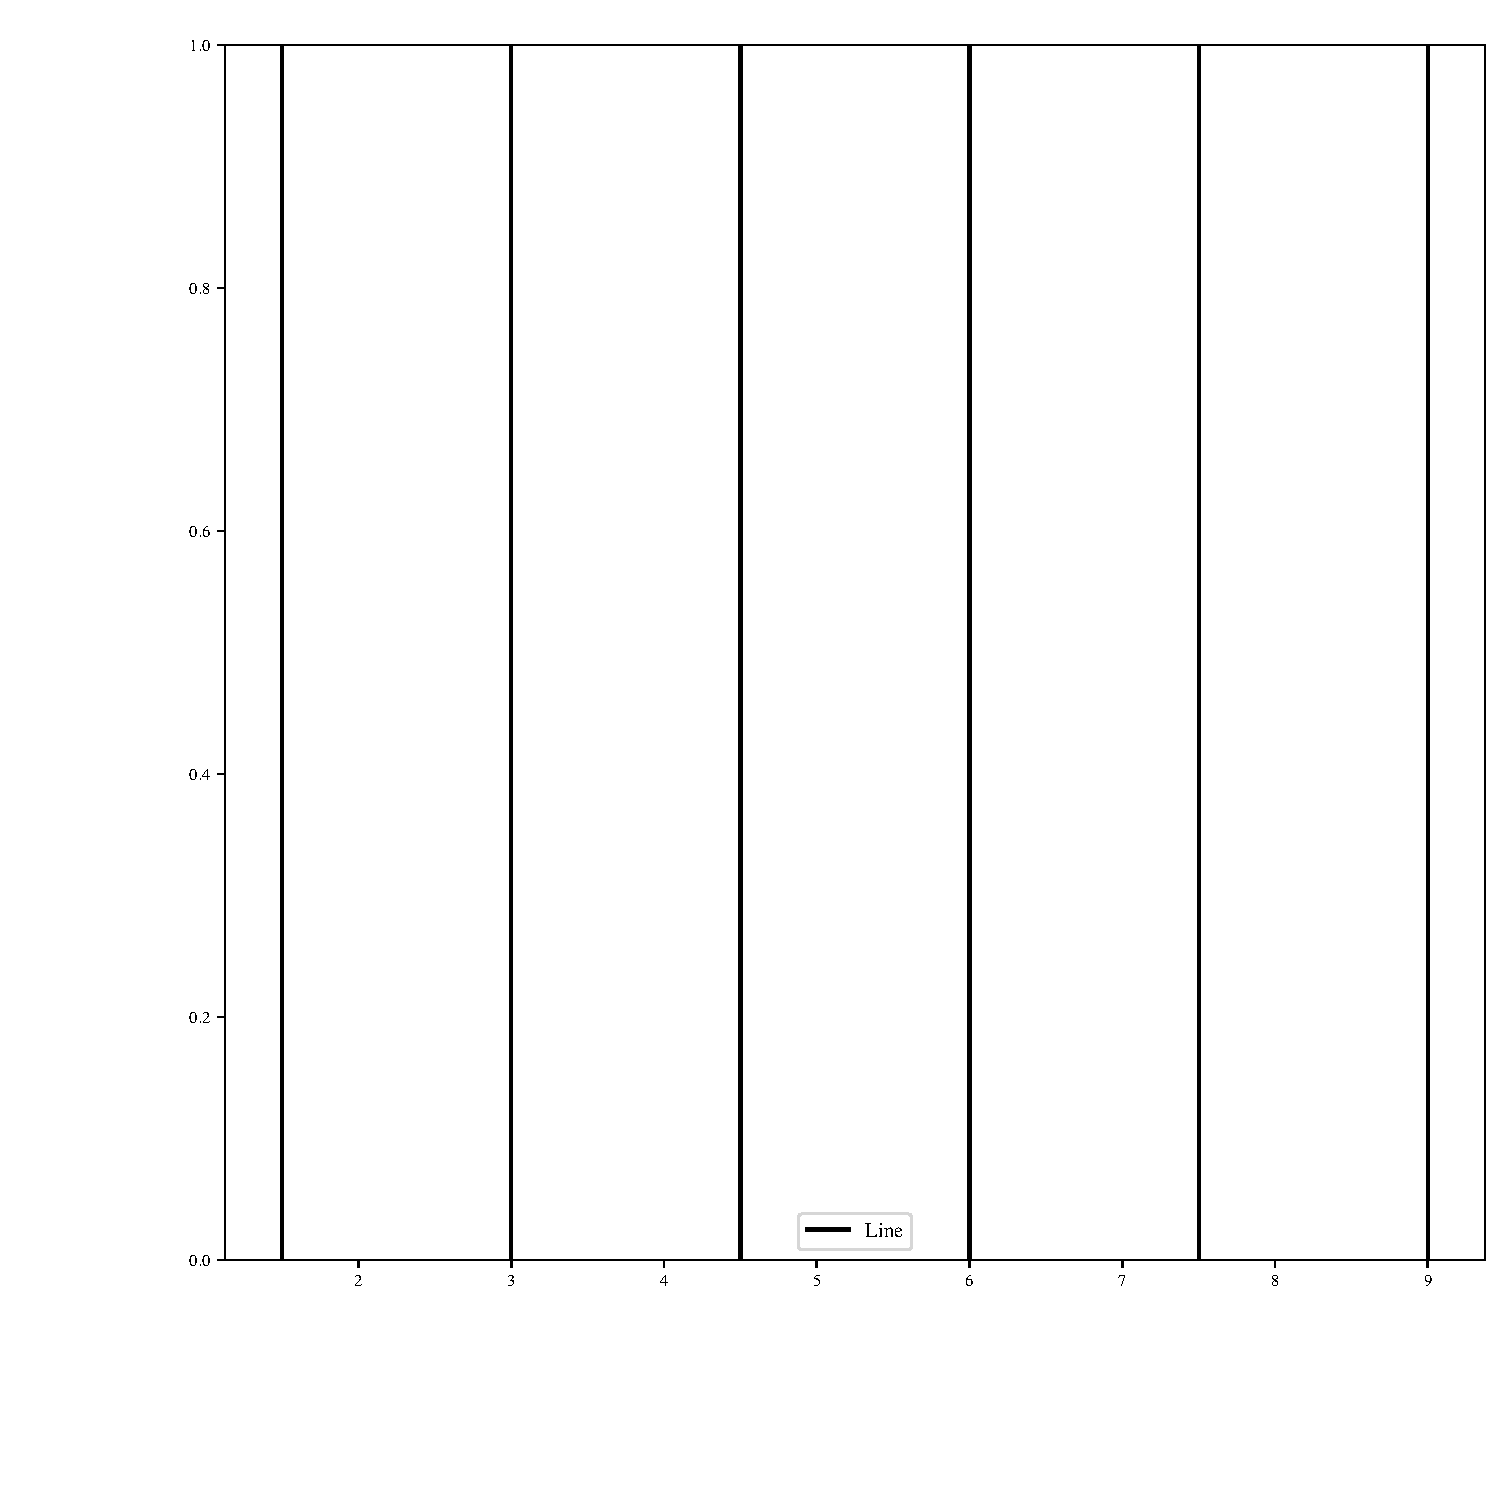
\includegraphics[width=.65\textwidth]{buffon.pdf}
\caption{Sample Buffon needle experiment. 100 needles are dropped on a 10 $\times$ 10 cm area with lines spaced 1.5~cm apart. If a needle lands on a line it is recorded and coloured blue, else it is red. This simulation gave a value of $\pi$ $\approx$ 3.10.}
\label{fig:buffon-needle}
\end{figure}

There are various different approaches to using the Monte Carlo method to obtain randomly sampled variables.
One analytical way of achieving this is the inverted sampling method.
The inverted sampling method can be summarised by the following steps for drawing a sample $X_i$ from an arbitrary PDF $p(x)$:

\medskip

1. Compute the \gls*{cdf} $P(x)=\int^{x}_{0}p(x')dx'$

2. Compute the inverse $P^{-1}(x)$

3. Obtain a uniformly distributed random number $\xi$

4. Finally, compute $X_i = P^{-1}(\xi)$

\medskip

If a given problem cannot use the inverted sampling method, as it may not be possible to get a PDF or analytically invert the CDF, then the rejection method can be used.
The rejection method is essentially a dart throwing method.
This means that points are drawn and compared to the function.
If the point lies under the function then the point is accepted, if it lies above the function then it is rejected.
For example, if a function, $f(x)$ that does not have an analytical PDF, we can use a PDF $p(x)$ such that $f(x) < cp(x)$ where c is a constant.
Therefore sampling from $p(x)$, and if the sampled point lies under $f(x)$ it is accepted, else it is rejected.
~\Cref{fig:picircle} shows an example of this process.

\begin{figure}[!ht]
    \centering
    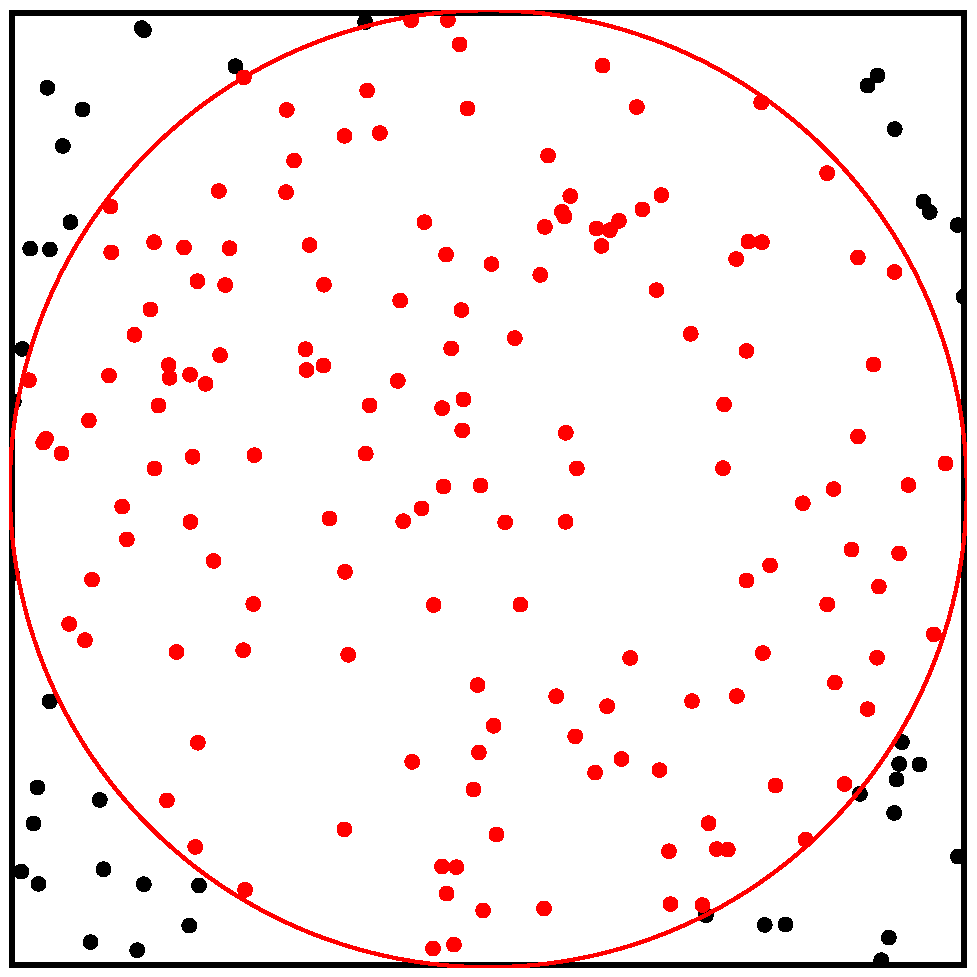
\includegraphics[width=0.35\textwidth]{picirc.pdf}
    \caption{Illustration of the rejection method for determining $\pi$ from the area of a circle inscribed within a square. The ratio of the area of the circle to the square is $\tfrac{\pi}{4}$. Thus the ratio of darts landing in the circle to those that land outside the circle is $\pi \approx \tfrac{4N_{inner}}{N_{total}}$, where $N_{total}$ is the total number of darts, and $N_{inner}$ is the total number of darts that land in the circle. Using 200 darts gave a value of $\pi \approx 3.12$}
    \label{fig:picircle}
\end{figure}


The Monte Carlo method is used in various different disciplines. Ranging from use in the financial sector to analyse investments and stocks by simulating the sources of uncertainty which affect their values~\cite{jackel2002monte,finaceprrof}, use in statistical analysis~\cite{wall2012practical}, and in modern computer generated images (see \cref{fig:ray-trace})~\cite{Kajiyarendering,Cookraytracing}. It is also widely used in astronomy~\cite{robitaille2011hyperion,harries2014torus} and medicine~\cite{valentine2011monte,campbell2015monte}, to simulate the propagation of radiation through scattering (turbid) media. This technique, \gls*{mcrt}, is what makes up the bulk of this thesis and is described in depth in the following sections.

\begin{figure}[!htb]
\centering
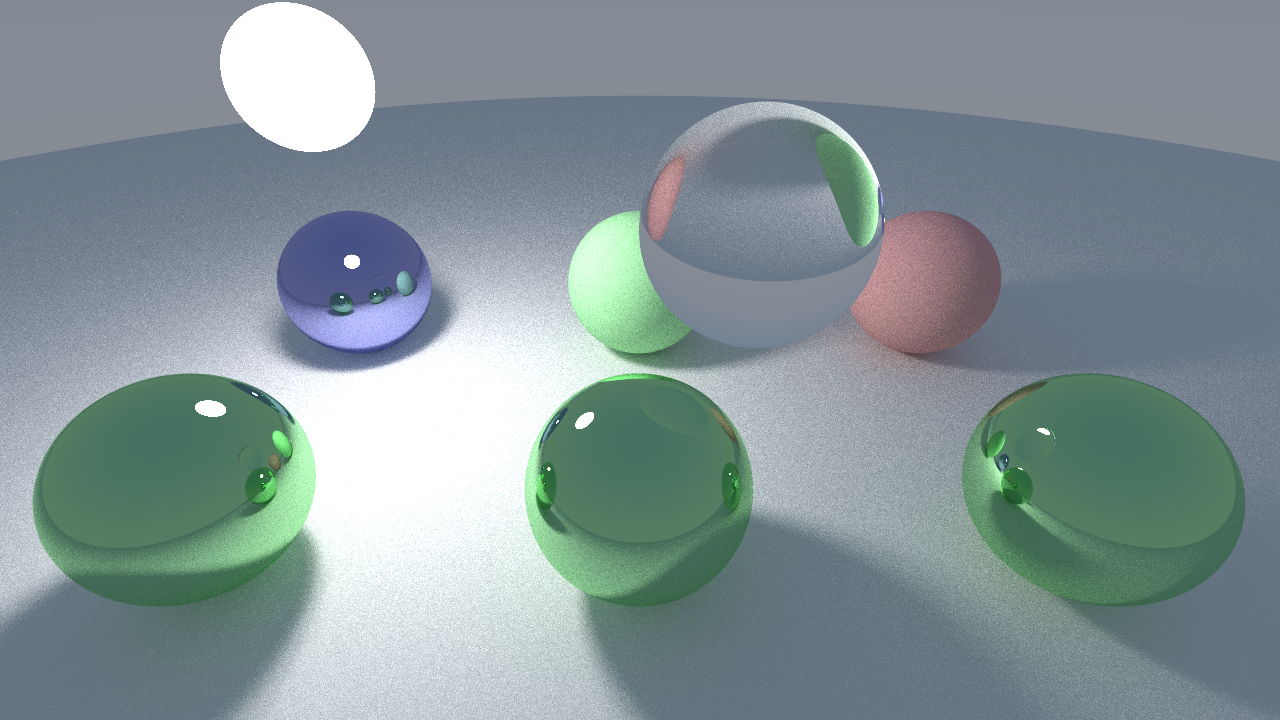
\includegraphics[width=.75\textwidth]{ray-tracing.png}
\caption{Computer generated imagery using ray tracing. The Monte Carlo method is used to ``compute radiance along ray paths between lights and the camera'', to generate CGI images~\cite{pharr2016physically}.}
\label{fig:ray-trace}
\end{figure}


\section{Synopsis and Thesis Objectives}
%sign post chapters

Again repeat first para -> talk about dev of MCRT and why use it i.e non invasive digital twin thing ilas mentioned. mcrt is flexable etc


Chapter two details the Monte Carlo radiation transport method that is used for the bulk of this thesis.
Presented in this chapter are details of the algorithm and various code details that underpin the whole thesis.
Details of speed up techniques such as parallelisation are also presented.
Finally the code is validated against other results.\\


Chapter three demonstrates details the tissue ablation model.
Discussion of the individual components of the model, alongside validation of the model against theoretical and experimental evidence is also presented.\\


Chapter four presents an adaptation to the regular Monte Carlo model so that it can model wave like properties of photons including diffraction and interference.
The new algorithm is validated against several theoretical expressions and experimental data.
Finally the algorithm is used to compare Bessel beams and Gaussian beam in highly turbid media, to determine which beam preforms better.\\


Chapter five details the modelling of a novel biomarker for cardiovascular disease, autofluorescence.
The theoretical groundwork for the biomaker is outlay-ed, along with discussion of how Monte Carlo radiation transport can model fluorescence.
Presented alongside this is ameombaMCRT, a Monte Carlo radiation transfer simplex algorithm used to determine concentrations of fluorophores in different layers of tissue for a given spectrum.\\
Chapter six details ....\\


Finally chapter seven concludes this thesis and presents possible future avenues of research that could be undertaken.